\documentclass[b5paper]{article}
%\usepackage[utf8]{inputenc}

%\usepackage{fontspec}
%\setmainfont{Linux Libertine O}

\usepackage{polyglossia}
\usepackage{amsmath}
\usepackage{multirow}
\usepackage{amsfonts}
\usepackage{amssymb}
\usepackage{breqn}
\usepackage[parfill]{parskip}
\usepackage{tikz}
\usepackage{float}
\usepackage{epstopdf}
\usepackage{color}
\usepackage{fontspec}
\usepackage{xunicode}
\usepackage{xltxtra}
\usepackage{fancyhdr}
\usepackage{expex}
\usepackage{bm}

\usepackage{subcaption}

\usepackage[left=1.65cm,right=1.65cm,top=2cm,bottom=2cm]{geometry}
%\chead{\textsc{\small }}
%\rhead{}
%\lfoot{}
%\cfoot{\thepage}
%\rfoot{}
%\pagestyle{fancy}

\makeatletter
\def\blfootnote{\gdef\@thefnmark{}\@footnotetext}
\makeatother

\setmainfont[Mapping=tex-text]{Linux Libertine O}

\newcommand{\todo}[2]{{\textcolor{red}{\bf [#1] #2 }}}
\newcommand{\note}[1]{{\textcolor{blue}{#1}}}

\newcommand{\ns}{{North Sámi }}


\title{Automatic Speech Recognition for  for \ns} 
\author{Peter Smit \\ \texttt{peter.smit@aalto.fi} \and Juho Leinonen \\ \texttt{juho.leinonen@aalto.fi} \and Mikko Kurimo\\ \texttt{mikko.kurimo@aalto.fi}  \\
[0.5cm]Department of Signal Processing and Acoustics, Aalto University\\}


\begin{document}

\maketitle

\begin{abstract} We have developed a Large Vocabulary Continous Speech Recognizer for \ns, an uralic langage that has little resources for speech technology available. Using only a limited audio data, 2,5 hours, and the \ns Wikipedia as language model we achieved n\% Letter Error Rate. With a language model based on the Trömso dataset we achieved n\% LER. To put this in perspective we also trained Finnish and Estonian systems with the same amount of data and compared those to state-of-the art systems in those languages.   \end{abstract}

\note{To be submitted to the Second International Workshop on Computational Linguistics for Uralic Languages, iwclul2016. Deadline 2nd November. `Papers should be up to 10 pages in length excluding references'}
\section{Introduction}

\ns is the largest of the nine Sámi languages with about 20 000 speakers. It belongs to the Uralic language family.

Like other languages in the Uralic language familiy, like Finnish and Estonian, it is highly morphological as the language uses independent suffixes extensively. This poses challenges for speech technology applications as the number of inflections, derivations and compoundings cause the size of the vocabulary to be enourmous, especially compared to the languages in the Indo-European family, which are most often researched. The great different number of words causes especially problems in the estimation of language models, which can not produce any words beyond those seen in the the training data. 

\ns is also an under-resourced language. There are little corpora of spoken and written language available, and financial resources to collect these data are limited. Even though there is active linquist research on \ns \todo{P}{Mention tromso and helsinki}, there are limitations to the expert resources avaible for speech recognition, such as pronunciation dictionaries. 

To combat the challenges of building an LVCSR system for an under-resourced language we have employed different techniques. First we used `found data' for building the acoustic and language models. For the acoustic model we needed to bootstrapped from a bigger related language (Finnish). For the language model we used subword units (morphs) to increase the coverage of the language.

To project a possible upper-bound on the recognition accuracies possible for \ns, we also have produced systems for Finnish and Estonian, using the same quantities of data for comparison. Comparing these to the state-of-the art systems for Finnish and Estonian will give a good estimate of the possible gains before more \ns data is gathered.

This work is an extension of \cite{leinonen2015}.

\section{Application}
The final application for the recognizer is to be deployed as part of a spoken dialogue system in the WikiTalk application \cite{wilcock2013wikitalk}. This is one part of the DigiSami project which ``is a research project at University of Helsinki which aims to support content generation of less resourced languages with the help of language technology''. Currently, the biggest dangers to Sami language are the disappearance of the traditional lifestyle and work of Sami culture, and emigration of Sami people from their old living areas. However, there are also studies and discussion on using new technologies to revitalize languages \cite{eisenlohr2004language}. In \cite{jokinen2014open}, the author describes revitalization for the \ns language using the WikiTalk application. In WikiTalk, the idea is to have users (children or adults) find out more about subjects that interest them by discussing with the humanoid robot Nao. They can ask for more information on the subject and then Nao will read them the related Wikipedia article \cite{jokinen2014multimodal}. Some related work using Nao with children is discussed in \cite{kruijff2012spoken}, where Nao would show exercises and plays, and with similar research as WikiTalk for Japanese Wikipedia \cite{kobayashi2011intelligent}




\section{ASR for under-resourced languages}
The majority of state-of-the art methods in Large Vocabulary Speech Recognition require big amounts of data and expertise. 

Firstly, a great number of high quality spoken utterances have to be collected and correctly transcribed. In case of a Speaker-Independent (SI) system, a system that can recognize anyone who speaks the target language, utterance from many different persons is needed. For a Speaker-Dependent (SD) system, a system that can only recognize the voice of the person that spoke the training data, many hours of voice and transcriptions are required.

The second required dataset is a large corpus of written text, preferably in the same style and domain as what should be recognized by the system. This corpus should at least contain all common words in their expected contexts in order to train a good language model.

Lastly, a normal speech recognizer needs a pronunciation dictionary. A list of all possible words with all their possible phonetic transcriptions. Also needed is a list of questions that separate the phonemes in different groups, this is used in acoustic model training to share probability distribution with decision tree clustering.

As none of the above data and expertise are readily avaibable for an underresourced language, alternatives have to be developed. In the case of transcribed audio data, a good resource would be audio books. Projects such as Librivox \todo{P}{Cite} have freely available audiobooks in many languages, although the quality varies. Using a temporary acoustic model and basic text processing techniques these audiobooks can be automatically segmented into sentence-long utterances that are suitable for training a minimal speaker-dependent model.

Also language data is often freely available online, though not necessary high-quality or in usable form. Web-scraping  \todo{P}{Cite}  can give a rudimentary dataset for training a language model. Also sites like wikipedia have often big collections of easily available text. The main problem with this `found' datasets is that the style and topic of the language data found does not match with the actual sentences spoken. Also, the datasets might contain foreign language segments, symbols or abbreviations that dillute the usability.

The pronuciation dictionary requires normally a great effort and linguistic expertise. One solution is to model the graphemes (letters) of the words directly, \todo{P}{Cite grapheme-to-sound} instead of using the actual phone they represent in the words. In languages such as English this would not give very good results as graphemes can have very different realizations. Consider for example the words `Tough' and `Though', in writing very similar words, but when spoken very different. In the Uralic languages studied here though, a grapheme-to-sound system would work very reasonable as in general every grapheme is only realized as a single distinct sound.

Lastly, the phoneme question set is a small dataset that can only be made by a language expert. Altough there are algorithms avaible that can replace this set altogther \todo{P}{Cite}, this is often undesirable as it effects the systems effectiveness. Another method is to take the phoneme set of a very closely related language, and alter it slightly to reflect the correct set for the target language. This can be often done with only minimal expert effort.

Eventhough there is a (partial) solution to all the expensive data needs, all these solutions do limit the resulting speech recognizer in different ways. In case of state-of-the art ASR systems, always more, higher quality, in domain speech and language data and expertise would improve the system signficantly (up to a certain point). There are however usable systems to be made in the under-resourced situation, with the most limiting factor being that SI systems are unattainable as the number of speakers is too low.




%	\section{UNUSED TEXT}
%	
%	This paper introduces a new speech recognizer for \ns, the largest of the nine Sami languages with about 20 000 speakers. \todo{Juho}{Cite}  Sami is a morphologically rich language in the Uralic group, and consequently it suffers from the same issues as Finnish speech recognition: inflection and compounding add a huge number of words to the lexicon. \ns is also an under-resourced language, so it is not feasible to collect enough data for a corpus that contains natural occurrences of all the different word forms. Another issue is the lack of expert help, for instance there is not enough resources to build a proper pronunciation dictionary for Sami, and therefore here, and in other model training phases, this paper introduces useful generalizations and unsupervised learning as techniques that could be applied to other under-resourced languages as well.
%	
%	Words are the most common unit for n-gram language models, and they work very well for analytic and isolating languages such as English. However, they are not the best choice for synthetic languages such as Finnish, Estonian or Sami. In these type of languages additional information is mostly added to the stem of the word, instead of using prepositions, postpositions or other parts of speech. Therefore, conferring information that might take many English words could be done with just one in Sami, for example TELL AN EXAMPLE. Thus, using segmented word fragments called morphs was tested as a language model unit for the recognizer. Morphs get their name from morpheme, which is the smallest grammatical unit of a language. In this paper both unsupervised and supervised learning for the optimal segmentation was tested, which resulted in morphs that represented grammatical segmentation, and ones that were generated to purely optimize the cost function of the segmentation tool, Morfessor Baseline 2.0 \cite{virpioja2013morfessor}. 
%	
%	Both these new language model units and words are compared to see which produces the best results in terms of error rates, both word error rate (WER) and letter error rate (LER). To make the results somewhat comparable, the total size of the language model will be restricted.
%	
%	\section{Used data}


\section{Acoustic modeling}
The Acoustic Modeling part of the speech recognizer was done with a standard Hidden Markov model with Gaussian mixture models as emission distribution (HMM-GMM). Mel Frequency Cepstral Coefficients were used as input features. 

The audio data is prepared by splitting the audio files (originally chapter length or similar) into sentence utterances. This is done by doing Baum-Welch forced alignment with a temporary speech recognition model. The temporary speech recognition model was created by taking a well trained Finnish model and mapping the Finnish phonemes to the one of the target language. In later iterations the best speech recognition model of the language was used to do the forced alignment again, resulting in a perfect split of training utterances.

The HMM-GMM model is trained using multiple iterations of Baum-Welch, maximum likelihood estimation. To manage the model complexity Gaussians were shared between different states using decision tree clustering.

Although there are different tuning possibilities in the acoustic model, specifically that control the number of parameters (Gaussians) in the model, the defaults were used as small experiments showed no improvements in different values. In Section~\ref{sec:compexp} the number of Gaussians for different models are reported.


\section{Language modeling}

\subsection{Words}

The main issue with using words as a language model unit for a synthetic language is that to decrease the out-of-vocabulary (OOV) rate to a manageable percentage, a huge lexicon is needed. Since OOV-rate is the minimum WER possible, a OOV-rate much less than 10\% would be necessary. For an English speech recognizer this can be achieved with already with 20 000 words for OOV-rate of 2.4-2.7\% and with a vocabulary of 40 000 words OOV-rate less than one percent is achieved \cite{woodland19951994}. In contrast, a Finnish recognizer needs a 410 000 word vocabulary to have an OOV-rate of 4.0-7.3\% \cite{hirsimaki2006unlimited}.

\subsection{Morphs}

Morphs get their name from morphemes, but here they are treated as just word fragments. The size of a word can be anything from a single letter to a whole word. While with words collecting them to a lexicon is a simple task of just gathering every individual word, and if need be limiting by maybe amount of occurances, a special tool is used to gathering from a corpus and then segmenting to them.

\subsubsection{Morfessor}

Morfessor is tool that applies machine learning principles to segment text into smaller fragments, with the main application being segmenting words into morphs \cite{creutz2007unsupervised}. The three components of a Morfessor are the model, cost function, and training and decoding algorithms. The model contains the lexicon: properties of the morphs, the written form of the morph itself and its frequency, and the grammar: how the morphs can be combined into words. Morfessor cost function is derived from a MAP estimation with the goal of finding the optimal parameters $\bm{\theta}$ given the observed training data $\bm{D}_W$:

\begin{equation}
\bm{\theta}_{MAP}=\operatorname*{arg\,max}_{\theta}P(\bm{\theta}|\bm{D}_W)=\operatorname*{arg\,max}_{\theta}P(\bm{\theta})P(\bm{D}_W|\bm{\theta}).
\end{equation}

The cost fuction to minimize becomes the minus logarithm of the product

\begin{equation}
L(\theta, D_W)=-log p(\theta)-log p(D_W|\theta).
\end{equation}

The purpose of this is to generate a small set of morphs that represents the words in the training corpus compactly. If only letters were used as morphs the set of would be small but representing the corpus with individual words would be cumbersome. In contrast using whole words as morphs would result in a large set of morphs so the optimal solution is somewhere in between. However, individual letters are added to the morph set so even previously unseen words can always be segmented.

A greedy search algorithm is used to find the optimal segmentation of morphs for the training data. One word is selected at a time and all different segmentations are tried, with the one that best improves the unsegmented part chosen and applied to all the other words. When the best model is found it is used to segment the LM training corpus with the Viterbi algorithm. This result can be used to generate n-gram models with morphs as LM units.



\subsection{N-gram modeling}
We have trained a standard word-based ngram model with the SRILM toolkit as baseline. However, to combat the data sparsity, we also created morph-based language models, which has proven to be very beneficial for morph-based languages \todo{}{Cite our best morph papers, also lrej?}

A morph-based language model is created by first splitting the source text into morphological units. We used the Morfessor tool, which can create a statistical morphological segmentation in an unsupervised manner. This segmentation is used to create n-gram language models. A split in morphological units reduces the number of types in the lexicon, but requires a greater language model context to be as effective as a word model. In agglunative languages like most uralic languages, creating a morph model causes the out-of-vocabulary rate to decrease dramatically.

As normal language model tools have problems with (correctly backing off) deep n-gram language models, we also have used the specialized VariKN toolkit to create a different language model.

For decoding we have used the AaltoASR decoder, which is specialized in decoding morph-language models with deep contexts.


\section{Experiment setup}

\note{we don't have to explain acoustic modeling, language modelling etc. We do need to tell what recognizer we used (AaltoASR) and what features it has (MFCC's, Gaussian-mixture HMM's, type of decoder). Same for language modeling tools}


The system the experiments were carried out on was AaltoASR \cite{hirsimaki2009importance}\cite{pylkkonen2005efficient}. It uses context-dependent triphones with diagonal Gaussian mixture models (GMM) as emission distributions and the speech features itself are extracted with Mel-frequency cepstral coefficients (MFFCs). Variable length n-grams are used for language modelling generated with both SRILM and VariKN \cite{siivola2007growing}\cite{siivola2007morfessor}. The decoder was a one-pass using token passing principles and hence time-synchronous. In addition, beam search complemented with a language model look-ahead is applied \cite{ortmanns1997look}.

%
%\subsection{Acoustic modelling}
%
%Aalto university's speech recognizer is like most speech recognizers in the sense that it uses hidden Markov models (HMM) to model triphones which have use as their emission distributions Gaussian mixture models (GMM). In Finnish, which is a phonetic language, the phonemes of the triphones are generated by just assuming that every letter represents a single individual phoneme. Based on this assumption a lexicon is built. This approach is also used for Sami since it too is a phonetic language and there are not enough resources for building a proper pronunciation dictionary. 
%
%\subsection{Language modelling}
%
%Maybe just a little bit of something, most in the actual section.
%
%
%\subsection{Decoding}
%
%The decoder used in AaltoASR is a "one-pass time-synchronous decoder using re-entrant prefic-tree and token passing principle". It is optimized for Finnish but otherwise language independent. Since the main language model units in Finnish speech recognition are morphs, one problem with the decoding becomes the context-dependent phonemes at the morph boundaries, and the need create a specific model for word boundary prediction. Other issue with Finnish are the double letters for which duration modelling needs to be applied. To limit the amount of transitioning modelling between context-dependent phonemes cross-word network is embedded in the search network. \cite{pylkkonen2013towards}\cite{hirsimaki2006unlimited} All of these solutions will also be used for the decoder for Sami, since morphs will also be tried for it, and it as three different vowel lengths and double consonants. A language model lookahead is also implemented to use the LM probabilities as soon as possible to prune unlikely hypothesis before applying the full computationally heavier language model. This study suggests this length, we will use this. since morphs.
%
%\section{Language modelling}
%
%n-gram, lexicon, words, morphs, morfessor. 
%
%N-gram word models are the most popular method for language modelling. They will also be used here, except using morphs instead of words will also be tested. Since in Sami the amount of word types rises very quickly with increasing corpus size (maybe tests about this with the larger corpus?), limiting the vocabulary might become needed, so tests are done to see its effect on the error rates, and n-gram amounts (speed). For segmenting words into morphs both supervised and unsupervised methods are tested.
%


%\section{Dealing with under-resourced ness}



%\subsection{Lexicon /\ pronunciation dictionary}
%
%maybe more carefully if needed. These people might actually want to see the letter-to-IPA-AaltoASR phoneme table?
%
%\begin{table}[h!]
%\caption{\ns alphabet and its representation in AaltoASR.\label{tab:graphemes}}
%\begin{center}
% \begin{tabular}{||c c c||} 
% \hline
% Sami & IPA & AaltoASR phoneme \\ [0.5ex] 
% \hline\hline
% A a & /\textipa{A}/ & a \\ 
% \hline
% Á á & /\textipa{a}/ & ä \\
% \hline
% B b & /\textipa{b}/ & b \\
% \hline
% C c & /\textipa{ts}/ & ts \\
% \hline
% Č č & /\textipa{tS}/ & C \\
% \hline
% D d & /\textipa{d}/ & d \\
% \hline
% Đ đ & /\textipa{D}/ & D \\
% \hline
% E e & /\textipa{e}/ & e \\ 
% \hline
% F f & /\textipa{f}/ & f \\
% \hline
% G g & /\textipa{g}/ & g \\ 
% \hline
% H h & /\textipa{h}/ & h \\
% \hline
% I i & /\textipa{i}/ & i \\
% \hline
% J j & /\textipa{j}/ & j \\
% \hline
% K k & /\textipa{k}/ & k \\
% \hline
% L l & /\textipa{l}/ & l \\
% \hline
% M m & /\textipa{m}/ & m \\
% \hline
% N n & /\textipa{n}/ & n \\
% \hline
% Ŋ ŋ & /\textipa{N}/ & N \\
% \hline
% O o & /\textipa{o}/ & o \\ 
% \hline
% P p & /\textipa{p}/ & p \\
% \hline
% R r & /\textipa{r}/ & r \\ 
% \hline
% S s & /\textipa{s}/ & s \\
% \hline
% Š š & /\textipa{S}/ & S \\
% \hline
% T t & /\textipa{t}/ & t \\
% \hline
% Ŧ ŧ & /\textipa{T}/ & T \\
% \hline
% U u & /\textipa{u}/ & u \\
% \hline
% V v & /\textipa{v}/ & v \\
% \hline
% Z z & /\textipa{dz}/ & z \\
% \hline
% Ž ž & /\textipa{dZ}/ & Z \\ [1ex]
% \hline
%\end{tabular}
%\end{center}
%\end{table}
%
%


\section{\ns ASR evaluation} 
\begin{table}[h!]
\begin{tabular}{ll}
Dataset & Training data\\
Female & 2.5 hours\\
Male & 3.5 hours\\
\end{tabular}
\end{table}

\begin{figure}[h!]
\centering
\begin{subfigure}[b]{.4\textwidth}

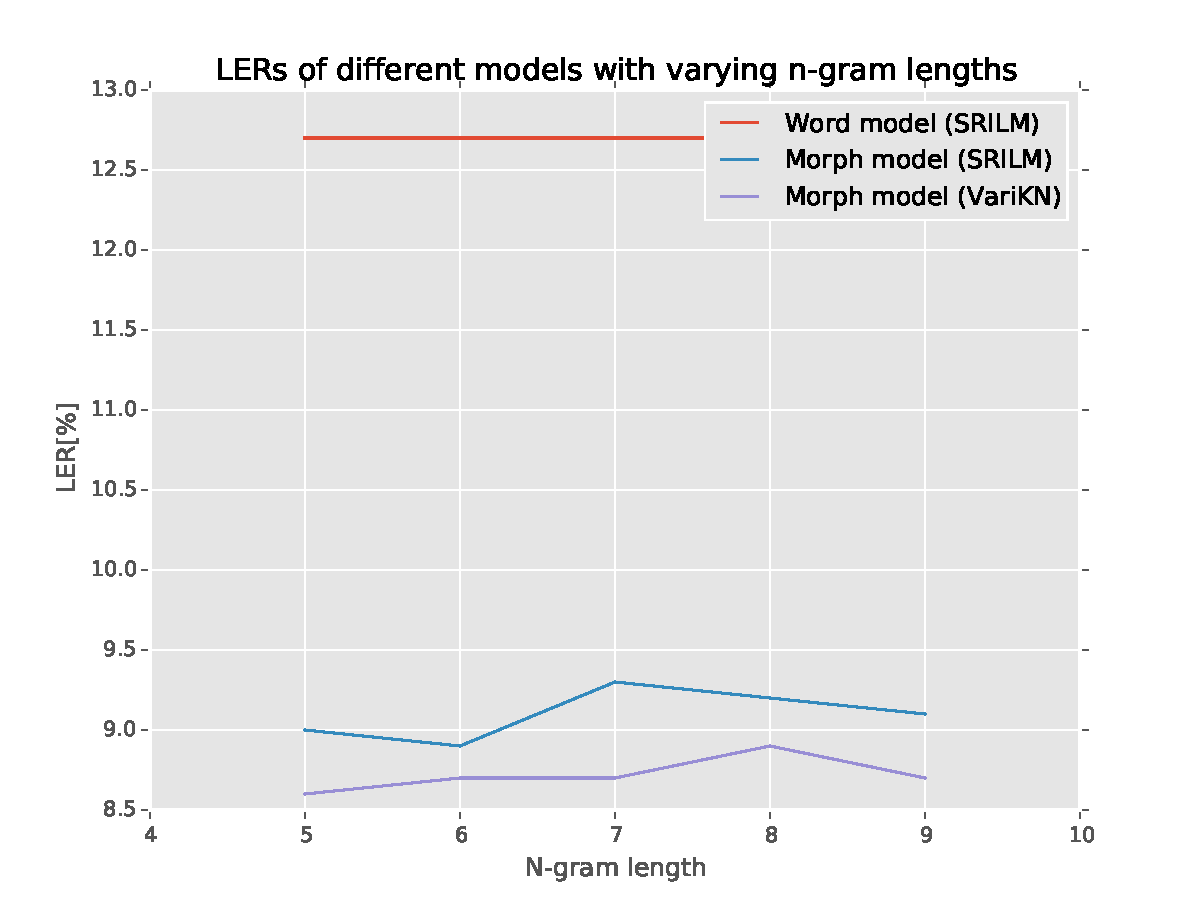
\includegraphics[width=\textwidth]{figures/smeF-complete_wikipedia-ler}
\caption{Female data - letter error rate}
\end{subfigure}~
\begin{subfigure}[b]{.4\textwidth}
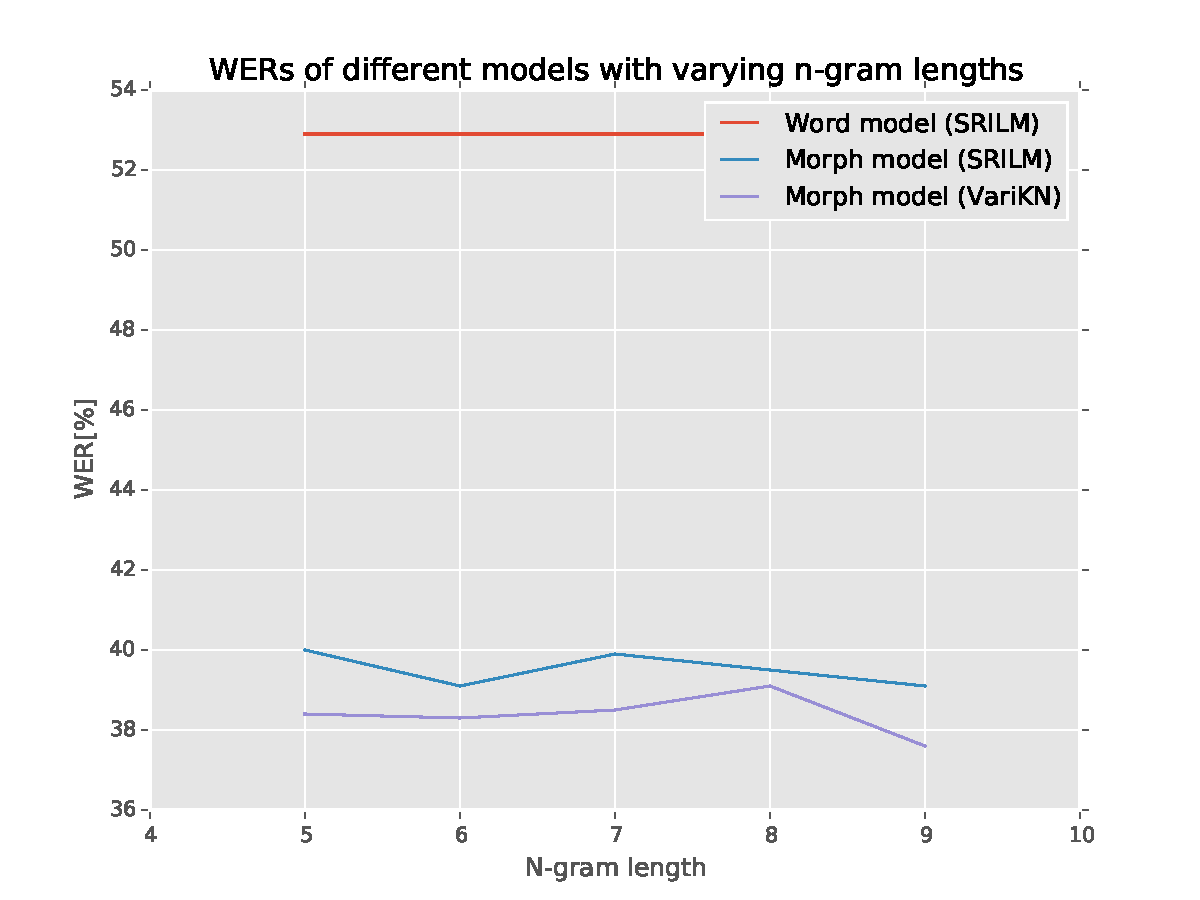
\includegraphics[width=\textwidth]{figures/smeF-complete_wikipedia-wer}
\caption{Female data - word error rate}
\end{subfigure}

\begin{subfigure}[b]{.4\textwidth}
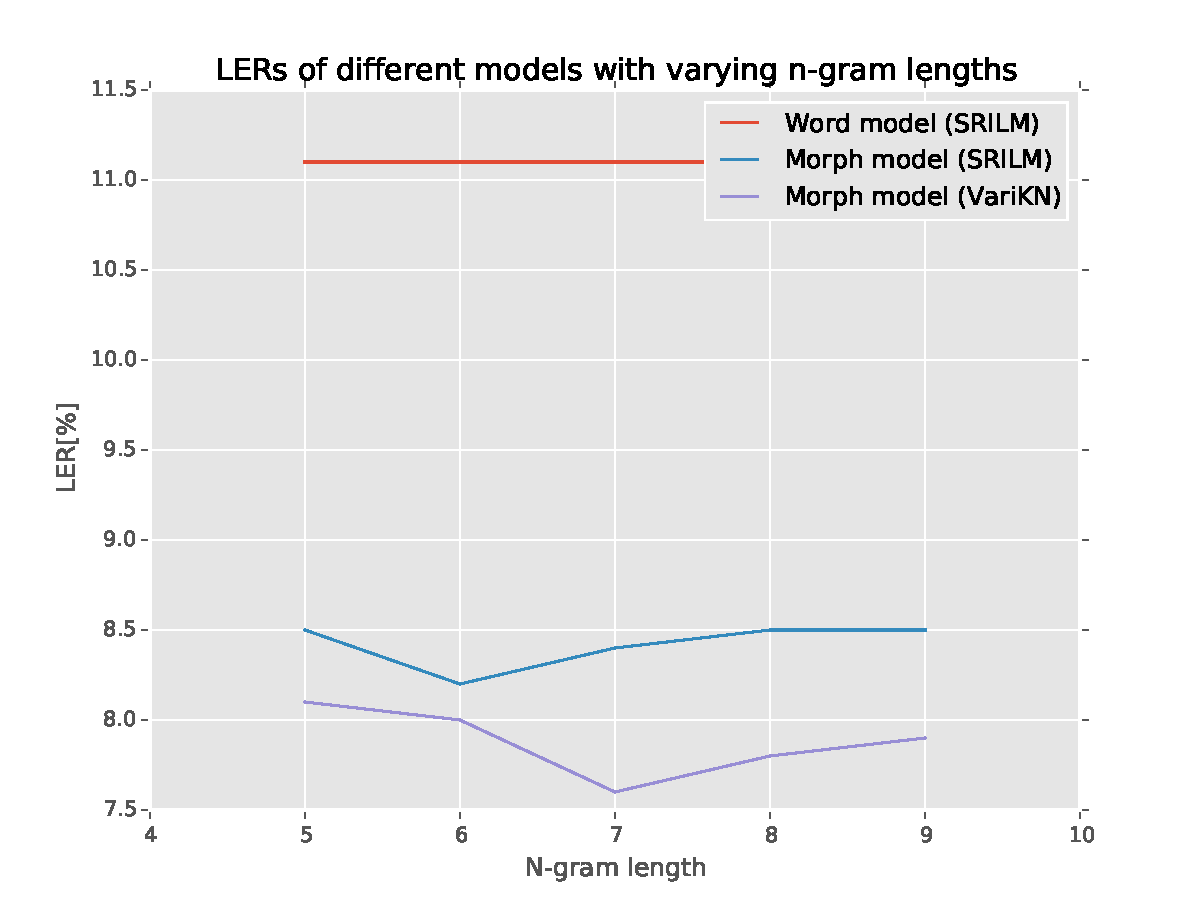
\includegraphics[width=\textwidth]{figures/smeM-complete_wikipedia-ler}
\caption{Male data - letter error rate}
\end{subfigure}~
\begin{subfigure}[b]{.4\textwidth}
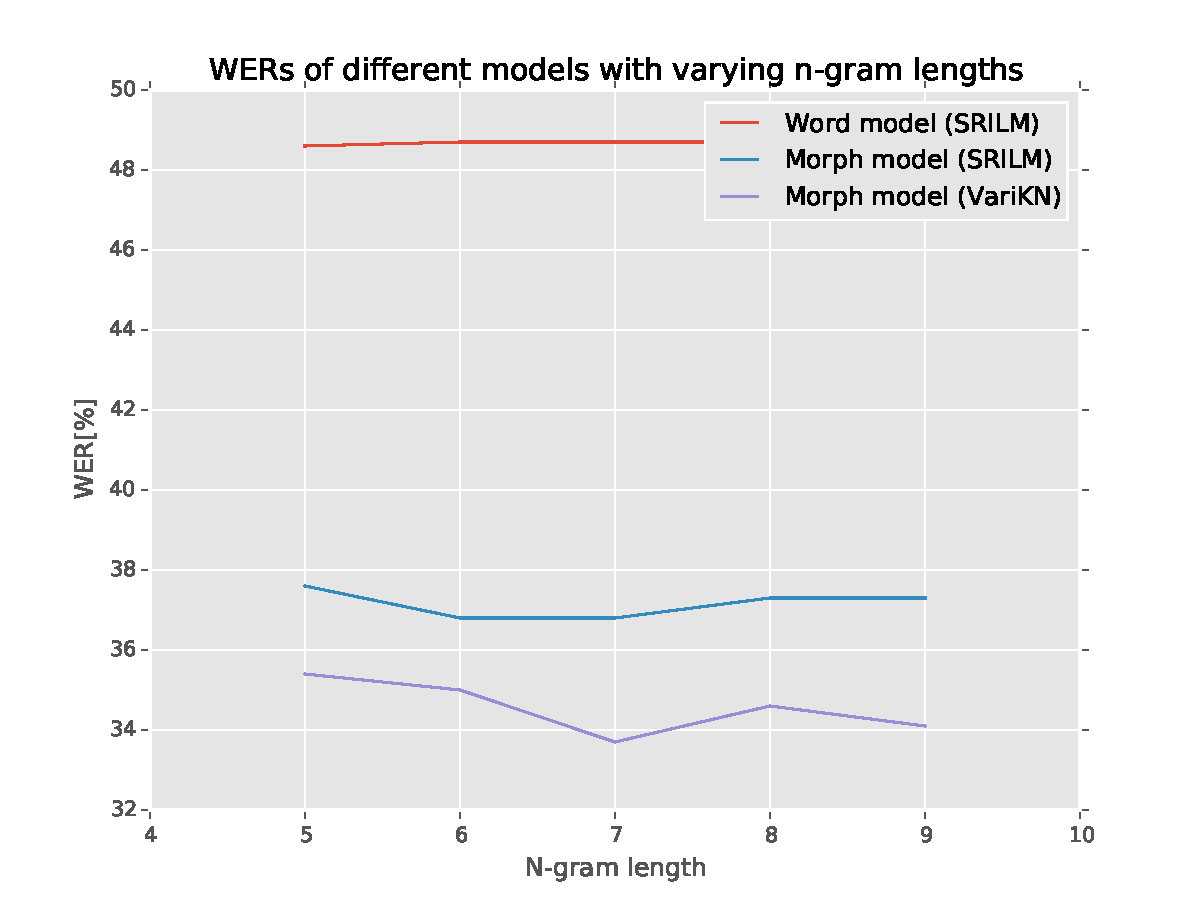
\includegraphics[width=\textwidth]{figures/smeM-complete_wikipedia-wer}
\caption{Male data - word error rate}
\end{subfigure}

\end{figure}

\section{Comparsion of low-resource systems for multiple languages}
\label{sec:compexp}
To compare the results of the \ns recognizer with recognizers in different languages we first trained speaker dependent models for both Finnish and Estonian audiobooks. The available audio datasets are described in Table~\ref{tbl:amdatacomp} and the available text corpora in Table~\ref{tbl:lmdatacomp}.


\begin{table}[h!]

\begin{tabular}{llllr}
 & \textbf{Language} & \textbf{Gender} & \textbf{Title} & \textbf{Amount}\\
EstF & Estonian & Female &Nils Holgerssoni imeline teekond läbi Rootsi  & 16 hours \\
EstM & Estonian & Male & Würst Gabriel ehk Pirita kloostri wiimsed päewad & 6 hours \\
FinF & Finnish & Female & Syntymättömien sukupolvien Eurooppa & 12 hours\\
FinM & Finnish & Male & Seitsemän veljestä & 13 hours\\
SmeF & \ns & Female & & 3.3 hours  \\
SmeM & \ns & Male & & 4.6 hours \\
\end{tabular}
\caption{Audio data for the trained speaker dependent systems\label{tbl:amdatacomp}}
\end{table}

\begin{table}[h!]

\centering
\begin{tabular}{llrrr}
\textbf{Language} & \textbf{Source} & \textbf{\#sentences} & \textbf{ \#word tokens} & \textbf{\#word types}\\
Estonian & Wikipedia &  895k & 10M & 778k \\
 Estonian & newspaper+web+broadcast & 19M  & 229M  & \\
 Finnish & Wikipedia &  2.2M  & 22M & 1.5M \\
 Finnish & Kielipankki & 13M &  143M & 4.1M \\
 \ns & Wikipedia & 10k & 88k & 20k\\
 \ns & Tromsø & 990k & 12M & 475k\\
%Est_wiki & Estonian & Wikipedia &Nils Holgerssoni imeline teekond läbi Rootsi  & 16 hours \\
%Est_ & Estonian & Male & Würst Gabriel ehk Pirita kloostri wiimsed päewad & 6 hours \\
%FinF & Finnish & Female & Syntymättömien sukupolvien Eurooppa & 12 hours\\
%FinM & Finnish & Male & Seitsemän veljestä & 13 hours\\
%SmeF & \ns & Female & &  \\
%SmeM & \ns & Male & & \\
\end{tabular}
\caption{Language modeling data for the trained speaker dependent systems\label{tbl:lmdatacomp}}
\end{table}

The comparable system takes only 2.5 hours of audio data and a random 10.000 sentences of the wikipedia data set for each language. The systems are trained with a 6-gram varikn language model. The statistics in Table~\ref{tbl:lmdatacomp_small} show that the datasets are equal in amount of sentences, but not in numbers of word types and tokens. This is most likely because the \ns wikipedia has more stub articles that contain short sentences with similar words.


\begin{table}[h!]

\centering
\begin{tabular}{llrrr}
\textbf{Language} & \textbf{\#sentences} & \textbf{\#word tokens} & \textbf{\#word types}\\
Estonian &   10k & 108k & 41k \\
 Finnish &   10k  & 103k & 43k \\
 \ns &  10k & 88k & 20k\\
%Est_wiki & Estonian & Wikipedia &Nils Holgerssoni imeline teekond läbi Rootsi  & 16 hours \\
%Est_ & Estonian & Male & Würst Gabriel ehk Pirita kloostri wiimsed päewad & 6 hours \\
%FinF & Finnish & Female & Syntymättömien sukupolvien Eurooppa & 12 hours\\
%FinM & Finnish & Male & Seitsemän veljestä & 13 hours\\
%SmeF & \ns & Female & &  \\
%SmeM & \ns & Male & & \\
\end{tabular}
\caption{Reduced subsets of wikipedia data\label{tbl:lmdatacomp_small}}
\end{table}

The results of the small recognizers are shown in Table~\ref{tbl:resultssmallcomp}.

\begin{table}[h!]

\centering
\begin{tabular}{llrr}
\textbf{Language} & \textbf{Gender} & \textbf{Word Error Rate} & \textbf{Letter Error Rate}\\
Estonian & Female & 39.6 & 15.8 \\
Estonian & Male & 44.0 & 16.5\\
Finnish & Female & 25.2 &4.1 \\
Finnish & Male &  35.8 & 7.7 \\
\ns & Female & 37.5 & 8.5 \\
\ns & Male & 39.5 & 9.4 \\
\end{tabular}
\caption{Speech recognizer results for the smallest dataset with wikipedia + own data language model, 6gram Varigram-kn + 2gram lookahead model \label{tbl:resultssmallcomp}}
\end{table}


\begin{table}[h!]

\centering
\begin{tabular}{llrr}
\textbf{Language} & \textbf{Gender} & \textbf{Word Error Rate} & \textbf{Letter Error Rate}\\
Estonian & Female & 39.6 & 15.8 \\
Estonian & Male & 44.0 & 16.5\\
Finnish & Female & 25.2 &4.1 \\
Finnish & Male &  35.8 & 7.7 \\
\ns & Female & 37.5 & 8.5 \\
\ns & Male & 39.5 & 9.4 \\
\end{tabular}
\caption{Speech recognizer results for the smallest audio dataset with the bigger language model \label{tbl:resultssmallcomp}}
\end{table}


\todo{P}{Mention different number of Gaussians or remove reference in Acoustic Modeling section}
State of the art in Finnish \cite{hirsimaki2006unlimited} and Estonian \cite{kurimo2015modeling}
\section{Conclusions} 

\section{Acknowledgements} 
\todo{}{Add wikitalk/digisami?} \todo{}{Thank tromso/helsinki} \todo{Mikko}{Coin or any other projects?}
We acknowledge the computational resources provided by the Aalto Science-IT project.



\bibliographystyle{unsrt}
\bibliography{mybib} 

\end{document}